\begin{frame}{Wie funktionieren die Modelle?}
\small
\begin{tabularx}{\textwidth}{l X}
\toprule
Faster R-CNN & Ein Region Proposal Network schlaegt Bereiche vor; danach werden Regionen klassifiziert und Boxen verfeinert. \\
RetinaNet & Klassifiziert und lokalisiert direkt auf Feature Maps; Focal Loss betont schwierige Beispiele. \\
FCOS & Anchor-free: sagt Objektpositionen pro Feature-Map-Position ohne vordefinierte Anchor-Boxen voraus. \\
YOLOv8m & One-Stage-Detector mit optimierter Inferenz, Run-Artefakten und direkter Video-Pipeline-Anbindung. \\
\bottomrule
\end{tabularx}
\vspace{0.6em}
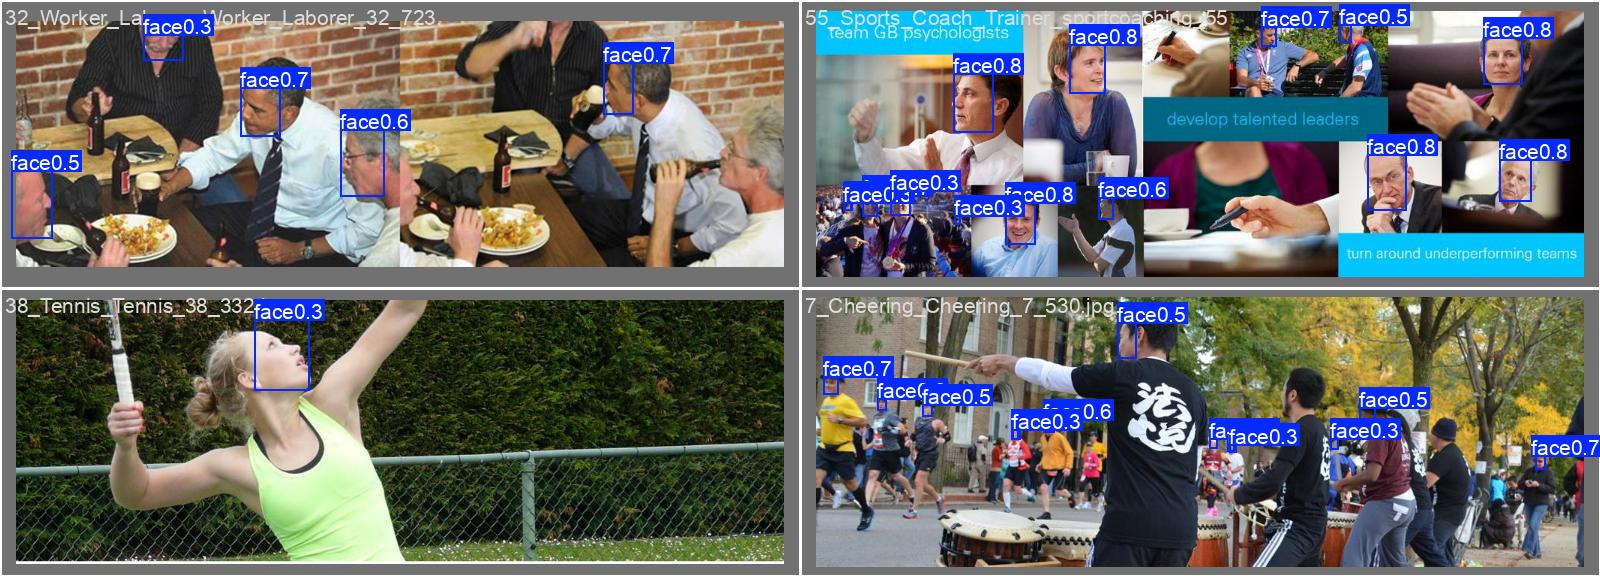
\includegraphics[width=\textwidth,height=0.28\textheight,keepaspectratio]{imglib/face_model_lab/yolo_val_predictions.jpg}
\end{frame}
